\documentclass[a4paper,11pt,oneside]{report}

\usepackage{url}
\usepackage{xspace}
\usepackage{times}
\usepackage{listings}
\usepackage{courier}
\usepackage{color}
\usepackage{geometry}
\usepackage{graphicx}

% defines

\def\libsklog{\texttt{libsklog}~\xspace}
\def\u{$\mathcal{U}$~\xspace}
\def\t{$\mathcal{T}$~\xspace}
\def\v{$\mathcal{V}$~\xspace}
\definecolor{shellbg}{RGB}{242,242,242}
\definecolor{shellbgsh}{RGB}{127,127,127}

% maketitle
\author{Paolo Smiraglia \\ \small{\url{paolo.smiraglia@polito.it}}}
\title{\libsklog \\ User Guide}
\date{Last Update:~\today}

% listings style
\lstset{ %
language=bash,
basicstyle=\scriptsize\ttfamily,
keywordstyle=\scriptsize\ttfamily,
%~ frame=trBL,
%~ frame=single,
frame=shadowbox,
rulesepcolor=\color{shellbgsh},
framerule=0pt,
stepnumber=2,
numbersep=15pt,
backgroundcolor=\color{shellbg},
showspaces=false,
showstringspaces=false,
showtabs=false,
tabsize=2,
captionpos=b,
breaklines=true,
breakatwhitespace=false,
title=\lstname,
escapeinside={\%*}{*)},
morekeywords={*,...}
}

\begin{document}

\maketitle
\tableofcontents

%%%%%%%%%%%%%%%%%%%%%%%%%%%%%%%%%%%%%%%%%%%%%%%%%%%%%%%%%%%%%%%%%%%%%%%%
%%%%%%%%%%%%%%%%%%%%%%%%%%%%%%%%%%%%%%%%%%%%%%%%%%%%%%%%%%%%%%%%%%%%%%%%
%%%%%%%%%%%%%%%%%%%%%%%%%%%%%%%%%%%%%%%%%%%%%%%%%%%%%%%%%%%%%%%%%%%%%%%%

\chapter{Introduction}

Libsklog is a library for C language which allows to perform secure
remote logging following the schema defined by B.Schneier and
J.Kelsey in \emph{Secure Audit Logs to Support Computer Forensics}.
This document illustrates how to install \libsklog under Linux
operating systems and how to configure the system enviroment to use it.
To get more information, to notify a bug, or generally to contact me
write at \url{paolo.smiraglia@polito.it}.

\section{The Schneier-Kelsey's model}

In Schneier-Kelsey's model, three entities are defined. They
consider a trusted machine \t (e.g. a server in a secure location),
an untrusted machine \u (potentially the victim of an attack) on
which the log entries are to be temporarily kept and a
moderately-trusted external verifier \v (e.g. an external auditor).
Moreover, a log entry creation scheme is well-defined (Figure \ref{fig:sk}).
With this type of scheme, the immediate identification of log
tampering (e.g. deletion of a log entry) becomes possible because
the log entries are linked in an \emph{hash-chain} by the element
$Y_{j}$. The integrity of logs is ensured by including an
HMAC field ($Z_{j}$) within the log entries and the confidentiality of
the logged data ($E_{K_{j}}(D_{j})$) is guaranteed thanks to the
usage of a symmetric cryptography mechanism. In SK when \v wants
to read the logs she requests and obtains the log entries from \u
and successively sends them to \t for validation and decryption.

\begin{figure}
\begin{center}
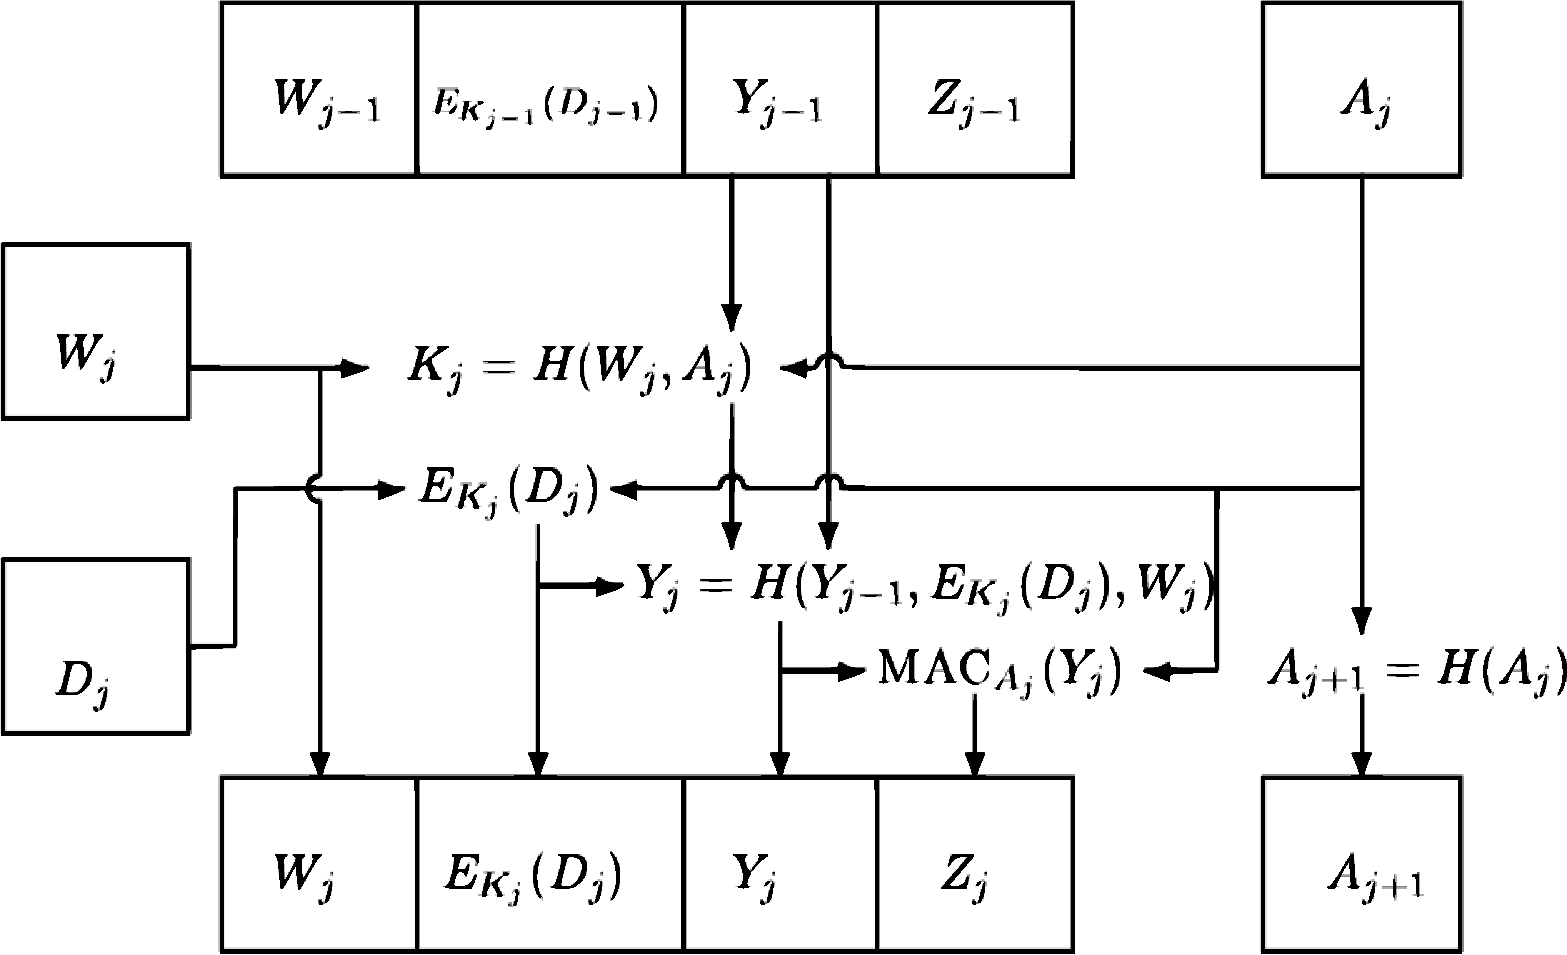
\includegraphics[scale=0.4]{images/sk-logentry-gen}
\caption{Schneier and Kelsey's log entry creation scheme.}
\label{fig:sk}
\end{center}
\end{figure}

%%%%%%%%%%%%%%%%%%%%%%%%%%%%%%%%%%%%%%%%%%%%%%%%%%%%%%%%%%%%%%%%%%%%%%%%
%%%%%%%%%%%%%%%%%%%%%%%%%%%%%%%%%%%%%%%%%%%%%%%%%%%%%%%%%%%%%%%%%%%%%%%%
%%%%%%%%%%%%%%%%%%%%%%%%%%%%%%%%%%%%%%%%%%%%%%%%%%%%%%%%%%%%%%%%%%%%%%%%

\chapter{Installation}

\libsklog allows to write applications which act as the actors \u, \t
and \v defined by Schneier and Kelsey. In this section is described
the \libsklog installation procedure and how to configure the
environment for
each component of Scneier-Kelsey
schema. All steps are described assuming that \libsklog installation
prefix is \texttt{/usr/local}.

%%%%%%%%%%%%%%%%%%%%%%%%%%%%%%%%%%%%%%%%%%%%%%%%%%%%%%%%%%%%%%%%%%%%%%%%
%%%%%%%%%%%%%%%%%%%%%%%%%%%%%%%%%%%%%%%%%%%%%%%%%%%%%%%%%%%%%%%%%%%%%%%%

\section{Get Sources and Install Library}

Before proceeding with the installation, the dependencies listed below
need to be resolved:

\begin{itemize}
%~ \item \texttt{Libtool}
%~ \item \texttt{Autoconf}
\item \texttt{OpenSSL $\ge$ 0.9.8}
\item \texttt{SQLite 3.x}
\item \texttt{libuuid-dev}
\item \texttt{libconfuse}
\end{itemize}

The first step is to get the source code of the library. Actually it's
only available on a Git repository hosted by GitHub.

\begin{lstlisting}
$ mkdir $HOME/temp
$ cd $HOME/temp
$ git clone https://github.com/psmiraglia/Libsklog.git libsklog
\end{lstlisting}

\begin{lstlisting}
$ cd $HOME/temp/libsklog
$ autoreconf --install --force --verbose
$ ./configure --prefix=/usr/local
$ make
$ make install (as root)
\end{lstlisting}

%%%%%%%%%%%%%%%%%%%%%%%%%%%%%%%%%%%%%%%%%%%%%%%%%%%%%%%%%%%%%%%%%%%%%%%%
%%%%%%%%%%%%%%%%%%%%%%%%%%%%%%%%%%%%%%%%%%%%%%%%%%%%%%%%%%%%%%%%%%%%%%%%

\section{Setup $\mathcal{U}$ Component}

TODO!

%%%%%%%%%%%%%%%%%%%%%%%%%%%%%%%%%%%%%%%%%%%%%%%%%%%%%%%%%%%%%%%%%%%%%%%%
%%%%%%%%%%%%%%%%%%%%%%%%%%%%%%%%%%%%%%%%%%%%%%%%%%%%%%%%%%%%%%%%%%%%%%%%

\section{Setup $\mathcal{T}$ Component}

TODO!

%%%%%%%%%%%%%%%%%%%%%%%%%%%%%%%%%%%%%%%%%%%%%%%%%%%%%%%%%%%%%%%%%%%%%%%%
%%%%%%%%%%%%%%%%%%%%%%%%%%%%%%%%%%%%%%%%%%%%%%%%%%%%%%%%%%%%%%%%%%%%%%%%

\section{Setup $\mathcal{V}$ Component}

TODO!


\chapter{Usage}



\end{document}
